\section{Application}
	Notre logiciel sert à analyser la sécurité d'un système à l'aide d'ADTrees, de leur construction et de leur visualisation.

	Lorem ipsum dolor sit amet, consectetur adipiscing elit. Integer tempus luctus ex, non fringilla nibh laoreet non. Nullam sed enim nec leo dapibus tincidunt. Nulla augue est, cursus tempus tristique eget, venenatis sed leo. Nam eget purus lacinia, porttitor dolor eu, consectetur turpis. Suspendisse sed viverra tellus. Aliquam malesuada sed magna mattis dapibus. Pellentesque eu molestie ligula. Pellentesque dictum ultricies sagittis. Ut semper, est vitae malesuada facilisis, magna velit laoreet lectus, semper suscipit sapien lacus sed nulla.

	Aliquam finibus est ac cursus cursus. Fusce in libero ut nisi laoreet sodales. Cras vestibulum nec nulla in consequat. In eget lacus ut ipsum placerat ultrices. Nam diam magna, fermentum aliquam libero at, ornare eleifend diam. Sed et mi eget arcu bibendum congue. Vivamus in enim mollis, blandit sem in, hendrerit tellus.


	\subsection{Interface}
		Regardez comment la figure \ref{fig:interface} est jolie.

		\begin{figure}
			\begin{center}
				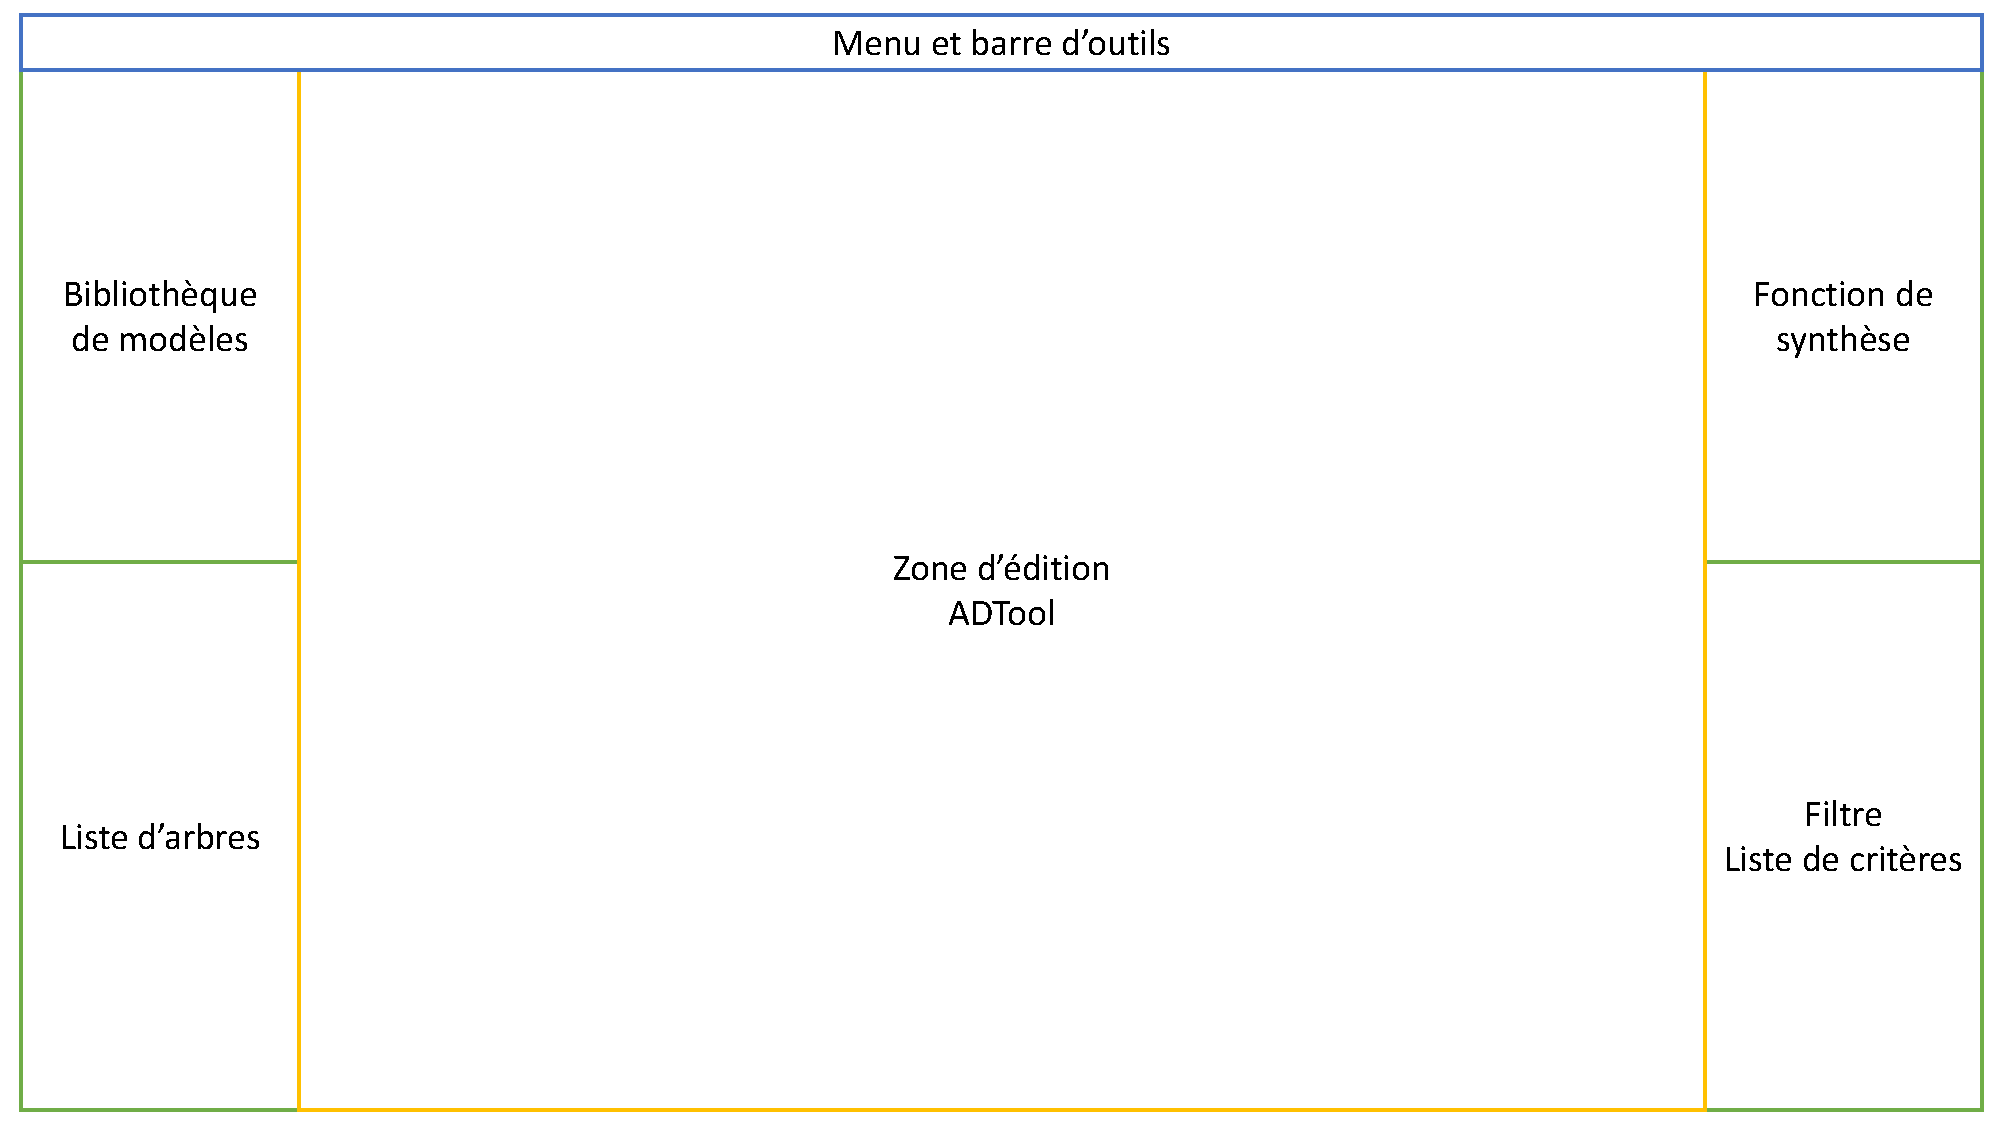
\includegraphics[width=1\textwidth]{figure/interface.pdf}
			\end{center}
			\caption{Là actuellement c'est la même figure que dans le rapport 1, on va changer ça.}
			\label{fig:interface}
		\end{figure}

		Maintenant on va expliquer l'interface et le fonctionnement général.

		Ensuite, on va détailler chaque module dans sa propre sous section. Chaque sous section contiendra une interface plus détaillée du module.

		Lorem ipsum dolor sit amet, consectetur adipiscing elit. Integer tempus luctus ex, non fringilla nibh laoreet non. Nullam sed enim nec leo dapibus tincidunt. Nulla augue est, cursus tempus tristique eget, venenatis sed leo. Nam eget purus lacinia, porttitor dolor eu, consectetur turpis. Suspendisse sed viverra tellus. Aliquam malesuada sed magna mattis dapibus. Pellentesque eu molestie ligula. Pellentesque dictum ultricies sagittis. Ut semper, est vitae malesuada facilisis, magna velit laoreet lectus, semper suscipit sapien lacus sed nulla.

		Aliquam finibus est ac cursus cursus. Fusce in libero ut nisi laoreet sodales. Cras vestibulum nec nulla in consequat. In eget lacus ut ipsum placerat ultrices. Nam diam magna, fermentum aliquam libero at, ornare eleifend diam. Sed et mi eget arcu bibendum congue. Vivamus in enim mollis, blandit sem in, hendrerit tellus.


	\subsection{Fichier projet}
	%	\begin{figure}
	%		\begin{center}
	%			
\includegraphics[width=1\textwidth]{figure/fichier.jpg}
	%		\end{center}
	%		\caption{Fichier}
	%		\label{fig:fichier}
	%	\end{figure}

		Mauris rhoncus tempor rhoncus. Vestibulum lacinia tincidunt sem ac auctor. Maecenas a lectus in nisi aliquet feugiat. Sed gravida laoreet maximus. Donec feugiat vestibulum neque sit amet mollis. Maecenas commodo luctus augue et molestie. Maecenas viverra semper massa, blandit commodo lacus blandit a. Proin sed euismod massa. Aenean nec nisl sed nisi mollis congue quis a nisi. Pellentesque habitant morbi tristique senectus et netus et malesuada fames ac turpis egestas. Suspendisse tincidunt euismod ipsum vitae commodo. Ut dapibus tellus nec libero egestas, eu venenatis dolor fermentum. Donec porttitor erat ante, at tincidunt lacus efficitur vitae.

		Vivamus elit urna, suscipit et nisi in, semper fringilla elit. In euismod cursus nunc quis tincidunt. Phasellus efficitur eleifend lacus, et pellentesque risus rhoncus vel. Phasellus in euismod lorem. Nam pulvinar aliquam metus a scelerisque. Etiam eget lectus ut felis porta ullamcorper. Aenean commodo at augue id pulvinar. Nunc efficitur elit est, id placerat sapien sodales nec. Etiam finibus at lacus nec viverra. Integer at vulputate mauris. Maecenas eget magna id tellus imperdiet finibus et in purus. Integer placerat ipsum a dui pellentesque, in lobortis lorem lobortis. In hac habitasse platea dictumst. 

	\subsection{Filtre}
		\begin{figure}
			\begin{center}
				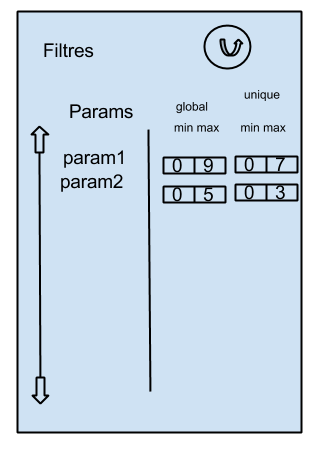
\includegraphics[width=0.25\textwidth]{figure/filtre.png}
			\end{center}
			\caption{Filtre}
			\label{fig:filtre}
		\end{figure}


		\begin{itemize}
		  \item bouton pour ajouter nouveau paramètre sur le filtre (par default : pas de filtre => pas de paramètres) 
			  \begin{itemize}
			  	 \item ajouter ouvre selection de paramétres : menu déroulant précisant les paramètres disponibles.
			  \end{itemize}
		  \item tous les paramètres ont à coté d’eux deux sections : une de filtre global et une de filtre unitaire. Dans le filtre global sont présentes deux cases, une nommée “min” et une nommée “max”. De même dans le filtre unitaire.
		  \item par défaut, les min sont moins l'infini et les max sont l’infini (pas de filtre)
		  \item il est possible d’inscrire des valeurs dans les cases “min” et “max” afin de réduire l’intervalle de sélection des branches de l'arbre.
		  \begin{itemize}
			  	 \item la section globale permet de conserver les branches de l’arbre dont la valeur totale du paramètre se trouve dans l’intervalle. (ex : entre 500 et 1000 euros au total)
			  	 \item la section unitaire permet de conserver les branches de l’arbre dont chacune des valeurs de chacune des feuilles se trouve dans l’intervalle. (ex : pas de dépenses de moins de 10 euros et pas de plus de 100 euros)
		  \end{itemize}
		  \item il est ainsi possible de combiner les critères de sélection (ex : entre 500 et 1000 euros au total et pas de dépenses de moins de 10 euros et pas de plus de 100 euros ; et le temps entre X et Y et ….)
		  \item barre de défilement pour les cas de surcharge de paramètres
		  \item possibilité d'activer ou désactiver les paramètres ( bouton a cocher)
		  \item bouton ``générer'' permet de créer un nouvelle arbre filtré en fonction des paramètres définie. Il est ouvert dans un nouvelle onglet de la section ADTool de l'interface. 
		  \item chaque arbre posséde son propre outil filtre. Lors de la génération, le nouvelle arbre posséde un outil filtre vide. 
		  \item le nouvel arbre posséde un commentaire : filtre depuis l'arbre X avec paramétre Y, heure, version. \ldots
		  \end{itemize}


	\subsection{Editeur de fonction}
		\begin{figure}
			\begin{center}
				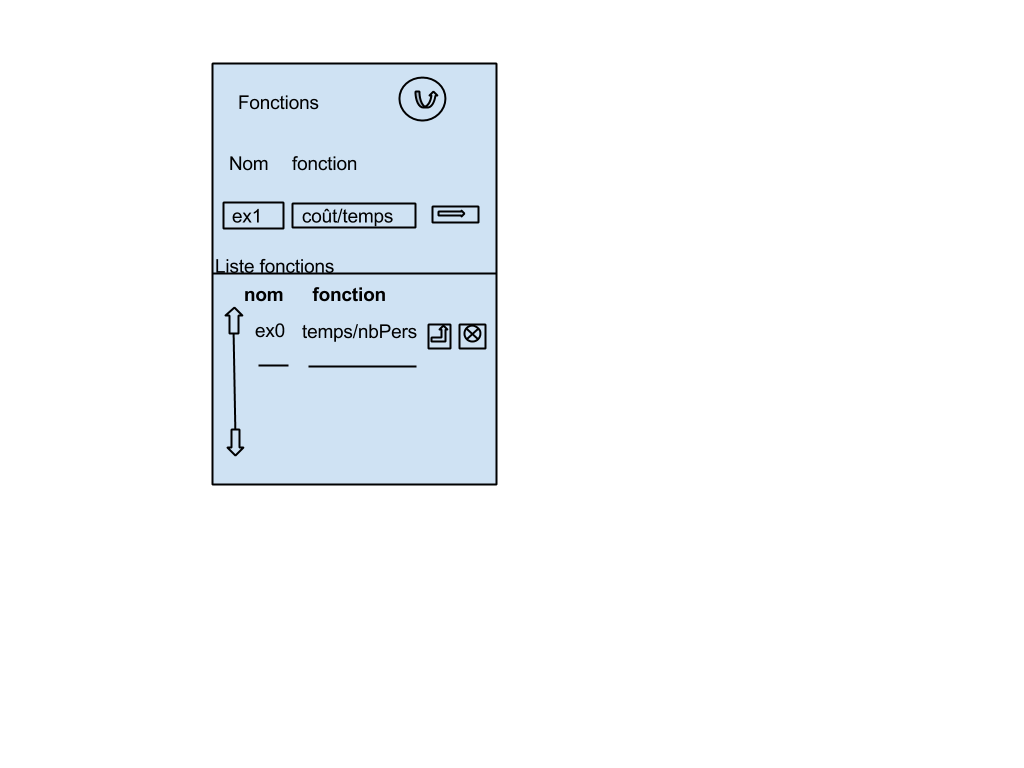
\includegraphics[width=0.25\textwidth]{figure/fonction.png}
			\end{center}
			\caption{Fonction}
			\label{fig:fonction}
		\end{figure}

		\begin{itemize}
			\item (présence préallable de 6 valuations de synthèse définies dans ADTool, et non instanciées par défaut. )
			\item décomposition en deux zones : une pour l'édition du nouveau paramètre et de sa fonction, et une pour le rappel des fonctions déjà existantes.
			\item Zone 1 : Présence d’un menu déroulant pour choisir laquelle des 6 valuation de synthèse est à instancier, et d'une zone textuelle pour écrire la fonction qu'on lui associe. La fonction est une fonction linéaire ou non, et qui prend en paramètres des valuations de l'arbre déjà définies (dans ADTool ou d'autres fonctions de synthèse). Bouton à coté pour valider la création. Si echec de la création (fonction non valable, etc.), message d'erreur donné par le guide (avec conseils éventuels).
			\item zone 2 : présence en dessous de la zone 1 d’une zone de rappel des fonctions de synthèse déjà instanciées. A coté de chacune d’entre elles il y a deux boutons : un pour modifier une fonction déjà créée, et un autre pour la supprimer.
			\item bouton “actualiser” en haut pour mettre à jour la liste des fonctions. \ldots
		\end{itemize}
		
		
		


	\subsection{Bibliothèque de modèles}
	%	\begin{figure}
	%		\begin{center}
	%			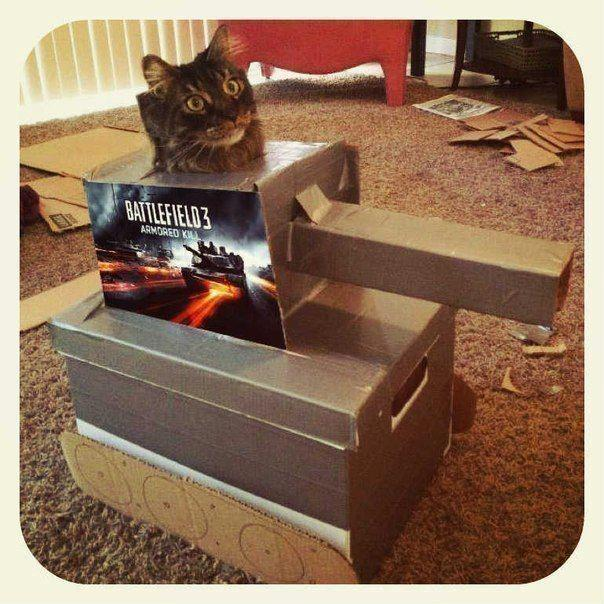
\includegraphics[width=1\textwidth]{figure/biblio.jpg}
	%		\end{center}
	%		\caption{Biblio}
	%		\label{fig:biblio}
	%	\end{figure}

		\begin{itemize}
			\item Le logiciel posséde une bibliothéque par défault
			\item la création d'un projet crée une nouvelle bibliothéque, copie de la bibliothéque par défault
			\item la bibliothéque est contenue dans le fichier projet de l'utilisateur. 
			\item Permet un accès facile à tous les arbres stockés
			\item bouton “actualiser” en haut pour mettre à jour la liste des fonctions.
			\item Regroupe les arbres par catégorie (par catégorie d’attaquant, de type d’attaque…), vue en arborescense. 	donner des types aux arbres stockés ?
			\item Permet d’y ajouter des éléments (géré automatiquement lors de la création dans un projet ?) Si non, bouton “ajouter” pour l’arbre courant. 
			\item Retirer des éléments : permet de retirer un élément et mettre à jour la bibliothèque, utile en cas d’arbre faux, ou considéré comme pas assez général pour servir de modèle. (cohérence avec l’ajout d’arbres)
			\item Pouvoir rechercher un arbre dans les modèles généraux (aussi rôle du guide) mais guide facultatif. Série de questions pour pouvoir sélectionner des modèles.
			\item Possibilité d'ajouter des arbres dans la bibliothéque par défault.\ldots
		\end{itemize}
		


	\subsection{Liste d'arbres}
	%	\begin{figure}
	%		\begin{center}
	%			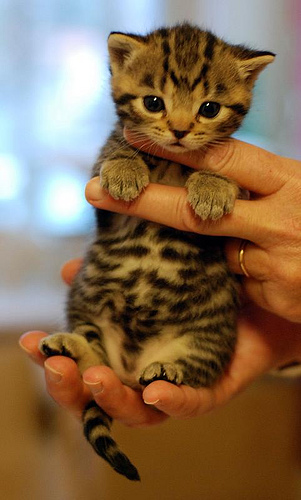
\includegraphics[width=0.5\textwidth]{figure/liste.png}
	%		\end{center}
	%		\caption{Liste}
	%		\label{fig:liste}
	%	\end{figure}


		\begin{itemize}
			\item Liste d'arbres générés par l'utilisateur puis sauvegardés sous différentes catégories/sous-catégories (arborescence)
			\item Au départ, une seule catégorie défaut
			\item  Création des catégories + possibilité d'affiner en sous-catégories
			\item Suppression d'une catégorie supprime tous les arbres compris dedans
			\item bouton “actualiser” en haut pour mettre à jour la liste des fonctions.
			\item Glisser/déposer les arbres pour les déplacer entre les catégories
			\item Possibilité de supprimer les arbres (renommer aussi ?)
			\item Double-clic pour ouvrir les arbres dans une fenêtre ADTool.\ldots
		\end{itemize}
		

	\subsection{Guide}
	%	\begin{figure}
	%		\begin{center}
	%			
\includegraphics[width=1\textwidth]{figure/guide.jpg}
	%		\end{center}
	%		\caption{Guide}
	%		\label{fig:guide}
	%	\end{figure}

		\begin{itemize}
			\item À activer dès la création du projet, possibilité de supprimer à tout moment 
			\item SAD peut aussi donner quelques conseils au début, genre raccourcis clavier), avec possibilité de désactiver
			\item Il peut aussi présenter le menu d'accueil du logiciel (Créer nouveau projet, etc)
			\item Donne des indications (genre Ouvre un nouveau projet) avec un bouton Suivant			
			\item SAD indique les erreurs (comme celles dans l'éditeur de fonctions), en gros toutes les exceptions levées par le logiciel\ldots
		\end{itemize}


	\subsection{Éditeur d'arbres}

		Attention: on ne parlera ici que de l'intéraction entre l'éditeur et les différents modules, pas de l'éditeur en lui même.
		Voir la section \ref{sec:adtool} pour voir nos améliorations.

		\begin{itemize}
			\item  Utilisation d'ADTool imbriqué dans l'IHM
			\item Une instance d'ADTool par arbre (possibilité d'ouvrir plusieurs onglets) : modèles, filtres, etc
			\item Chaque modification dans ADTool entraine une mise à jour de SAD
			\item Sauvegarde des fichiers par ADTool : ne pas laisser le choix du fichier, laisser seulement le fichier projet (en gros, l'arborescence d'arbres)\ldots
		\end{itemize}
